Una plataforma en la Nube para la gesti�n y localizaci�n de estacionamiento, Figura \ref{fig:ArquitecturaGeneralSAE}. Ser� capaz de ajustarse a las necesidades de las diferentes modalidades de estacionamientos p�blicos y privados del Distrito Federal como son estacionamiento con y sin pensiones, parqu�metros y valet-parking. Para los estacionamientos que ya cuenten con sistemas para gesti�n y/o automatizaci�n podr�n utilizar esta plataforma a trav�s de una API, para que su pueda ser visualizada por los potenciales usuarios finales. 

\begin{figure}[h]
	\centering
	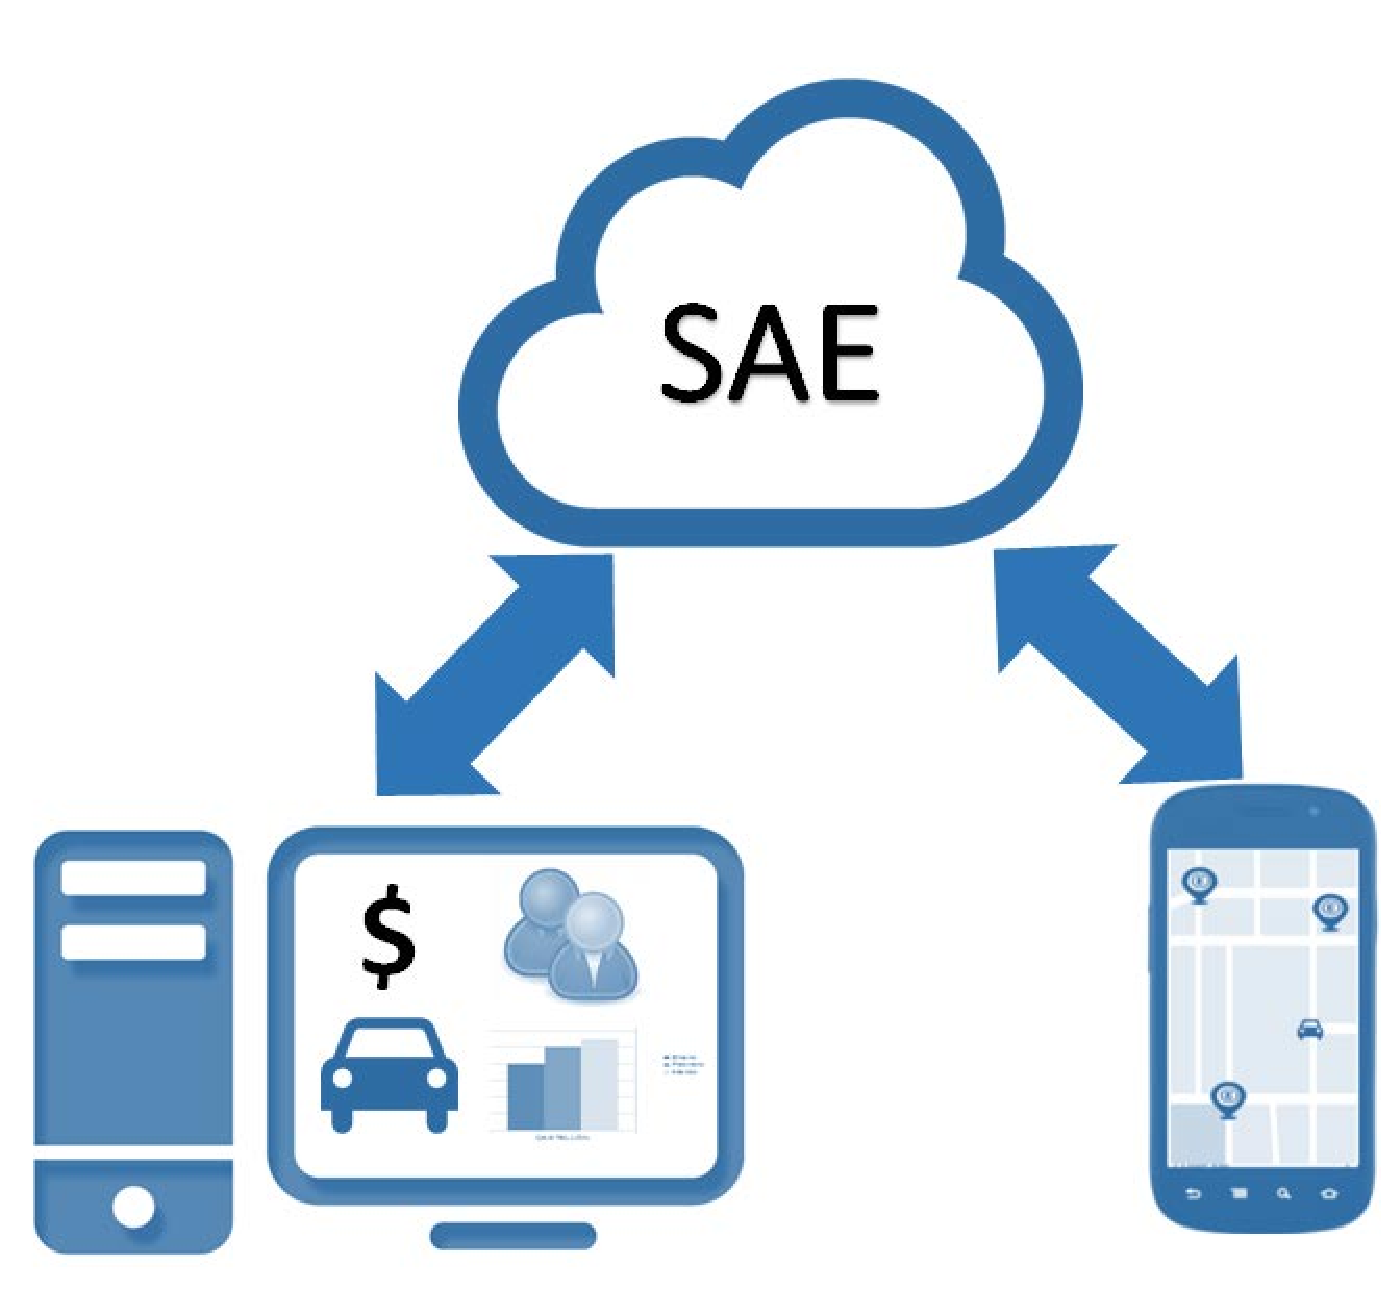
\includegraphics[scale=.25]{./estudioDeMercado/definicionDelProducto/source/arquitecturaSAE.pdf}
	\caption{Arquitectura general SAE}
	\label{fig:ArquitecturaGeneralSAE}
\end{figure}		 

La informaci�n de los estacionamientos en operaci�n podr� ser visualizada por los usuarios finales a trav�s de una app m�vil de manera f�cil. Esta mostrar� en un mapa la ubicaci�n de los estacionamientos cercamos, mostrando informaci�n relevante para el usuario, como es, n�mero de cajones disponibles, horarios, modos de cobro, tarifas, Etc. Figura \ref{fig:usuarioAppLocalizacion}
El usuario final podr� desde su app m�vil guardar el lugar donde se estaciono, visualizar su tiempo transcurrido, consultar la monto total por su uso, comunicarse v�a mensajes privados con el administrador, interactuar con todos los estacionamientos registrados en la plataforma.  


\begin{figure}[ht]
	\centering
	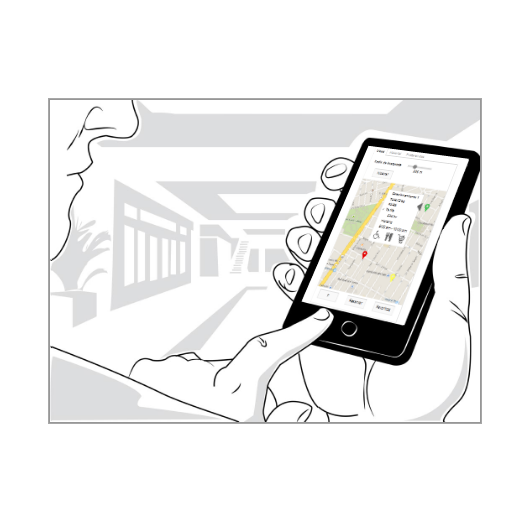
\includegraphics[scale=0.35]{./estudioDeMercado/definicionDelProducto/source/usuarioApp}
	\caption{App m�vil del usuario final}
	\label{fig:usuarioAppLocalizacion}
\end{figure}


\newpage
La Figura \ref{fig:EscenarioSAE} ejemplifica el escenario principal de uso de la plataforma.

\begin{figure}[ht]
	\centering
	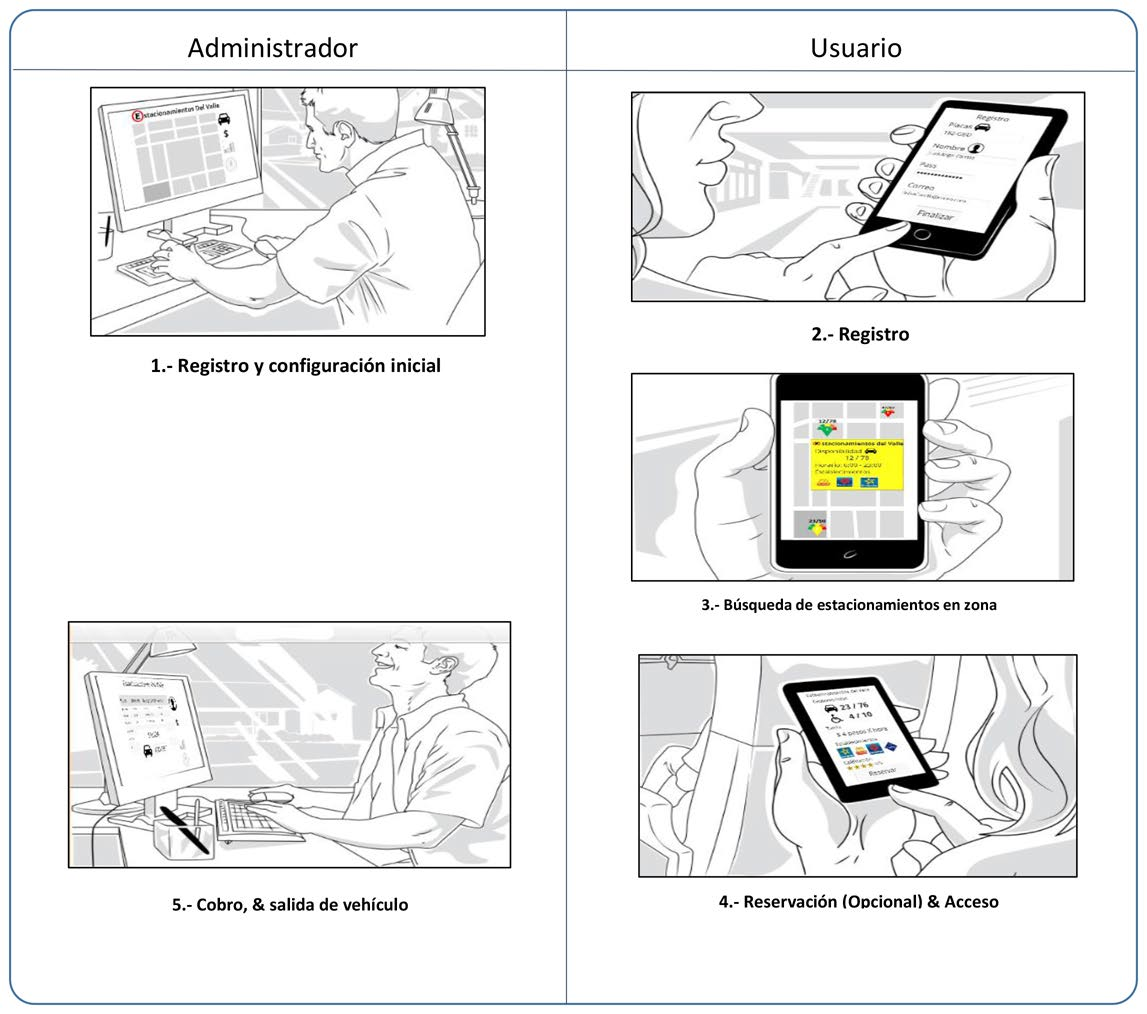
\includegraphics[scale=0.75]{./estudioDeMercado/definicionDelProducto/source/storyboard.pdf}
	\caption{Escenario de la plataforma}
	\label{fig:EscenarioSAE}
\end{figure}

 Las principales caracter�sticas del la plataforma son:
\begin{itemize}
	\item Configuraci�n f�sica
		\begin{itemize}
			\item N�mero de niveles
			\item N�mero de cajones
			\item Cajones para personas con capacidades diferentes.
			\item Ubicaci�n del estacionamiento 
			\item Horario de operaci�n
			\item Modalidad(Pensi�n, valet, normal)
			\item Publico o Privado
		\end{itemize}
	\item Control de entradas y salidas
	\item Control de usuarios
	\item Generaci�n de reportes
	\item Consultas
	\item Configuraci�n de tarifas
	\item Agregar servicios adicionales (lavado, aspirado, pulido, Etc.)
	\item API de integraci�n para otros sistemas
	\item App para usuario final
	
\end{itemize}